To demonstrate the usefulness, repeatability, and validity of the SAVAT metric and methodology, we will run the SAVAT benchmarks for several instruction pairs on some computing devices and measure the resulting EM emanations. The instructions listed in Tables~\ref{insts}~and~\ref{nios_insts} were used in the A/B alternation microbenchmarks as described in Section~\ref{sec:methodology} for each pairwise instruction combination. These lists include loads and stores serviced by different levels of the cache hierarchy, simple (ADD and SUB) and more complex (MUL and DIV) integer arithmetic, and the "No instruction" case where the appropriate line in our alternation code (Line \ref{TestInstA} or \ref{TestInstB} in Figure~\ref{pseudocode}) is simply left empty. The NIOS processor has only an L1 cache so LDL2 and STL2 are not applicable. 

\begin{table}[htb]%
  \small%
  \label{insts}%
    \caption{x86 instructions for our A/B SAVAT measurements.}%
    \begin{tabular}{lll}%
    \toprule
    & \textbf{Instruction} & \textbf{Description} \\
    \midrule
    LDM  & mov eax,[esi]        & Load from main memory \\
    STM  & mov [esi],0xFFFFFFFF & Store to main memory  \\
    LDL2 & mov eax,[esi]        & Load from L2 cache    \\
    STL2 & mov [esi],0xFFFFFFFF & Store to L2 cache     \\
    LDL1 & mov eax,[esi]        & Load from L1 cache    \\
    STL1 & mov [esi],0xFFFFFFFF & Store to L1 cache     \\
    ADD  & add eax,173          & Add imm to reg  \\
    SUB  & sub eax,173          & Sub imm from reg \\
    MUL  & imul eax,173         & Integer multiplication \\
    DIV  & idiv eax             & Integer division       \\
    NOI  &                      & No instruction \\
    \bottomrule
        \end{tabular}%
\end{table}%

\begin{table}[htbp]%
  \small%
  \centering%
    \begin{tabular}{lll}%
    \toprule
    & \textbf{Instruction} & \textbf{Description} \\
    \midrule
    LDM  & ldw  r21, 0(r21) & Load from main memory \\
    STM  & stw  r21, 0(r21) & Store to main memory  \\
    LDL1 & ldw  r21, 0(r21) & Load from L1 cache    \\
    STL1 & stw  r21, 0(r21) & Store to L1 cache     \\
    ADD  & addi r22,r22,173 & Add imm to reg  \\
    SUB  & subi r22,r22,173 & Sub imm from reg \\
    MUL  & muli r22,r22,173 & Integer multiplication \\
    DIV  & div  r22,r22,r22 & Integer division       \\
    NOI  &                  & No instruction \\
    \bottomrule
    \end{tabular}%
  \caption{NIOS instructions for our DE1 FPGA A/B SAVAT measurements.}%
  \label{nios_insts}%
\end{table}%

The systems tested are listed in Table~\ref{pc_specs}, along with relevant system properties such as CPU and memory clock rates, processor microarchitecture, and cache parameters. For the laptops and desktop, the benchmarks are run as single-threaded Windows 7 32-bit user mode console applications. No other user-mode applications were active and wireless devices were disabled to minimize interference with the intentionally generated signals. Aside from this, the systems were operating normally, meaning that any EM signals resulting from system processes and other OS activity would affect the received signal. For the FPGA, the benchmarks were run on a NIOS soft processor implemented on a DE1 Cyclone II FPGA board, with no memory management or operating system. No other logic was active on the FPGA. 

\begin{table*}[tb]%
  \scriptsize%
  \centering%
    \begin{tabular}{ccccc}%
    \toprule
    \textbf{System} & \textbf{Processor} & \textbf{Memory} & \textbf{L1 Data Cache} & \textbf{L2 Cache} \\
    \midrule
    Altera DE1 FPGA      & NIOS II ``fast'', 50 MHz  & 50 MHz SDRAM  & 4 KB, 1 way & None \\
    Dell Latitude C610   & Intel Pentium IIIM, 1 GHz  & 133 MHz DDR   & 16 KB, 4 way & 512 KB, 8 way \\
    Lenovo X61           & Intel Core Duo, 1.8 GHz & 333 MHz DDR2  & 32 KB, 8 way & 4096 KB, 16 way \\
    HP Pavilion tx2000   & AMD Turion X2, 2.3 GHz & 333 MHz DDR2  & 64 KB, 2 way & 1024 KB, 16 way \\
    Dell Optiplex 7010   & Intel Core i7, 3.4 GHz & 1600 MHz DDR3 & 64 KB, 2 way & 1024 KB, 16 way \\
    \bottomrule
    \end{tabular}%
  \caption{Measured FPGA, laptop, and desktop systems.}%
  \label{pc_specs}%
\end{table*}%


EM probe type, position, and orientation affect the strength of the received emanations. A small ``sniffer'' probe placed a few millimeters above components picks up signals from only the components near the probe, but receives these signals very strongly. On the other hand, placing a probe with a larger effective area far away ($>$~2~meters) will pick up signals from all the parts of the system, but is often not sensitive enough to pick up the weakest signals. Furthermore, the strength of the emanations from the x86 systems is much stronger than the emanations from the NIOS FPGA system. Therefore, two measurement setups were used. The first setup, shown in Figure~\ref{large_setup} was used for measurements and comparisons which did not involve the FPGA system. For these measurements, the periodic EM signal at the alternation frequency was measured using a 20~cm diameter magnetic loop antenna (AOR LA400) placed at a distance of 10~cm from the tested system. This antenna does not use a tuning capacitor and is terminated with a $50\Omega$ load, so it has a flat frequency response between $10~{\rm kHz}$ and $1~{\rm MHz}$. This will be referred to as the 20~cm loop setup. A recent paper illustrates a practical EM attack on implementations of the RSA and ElGamal algorithms using similar equipment and laptops~\cite{genkin_2014}. 

\begin{figure}[htb]
\centering
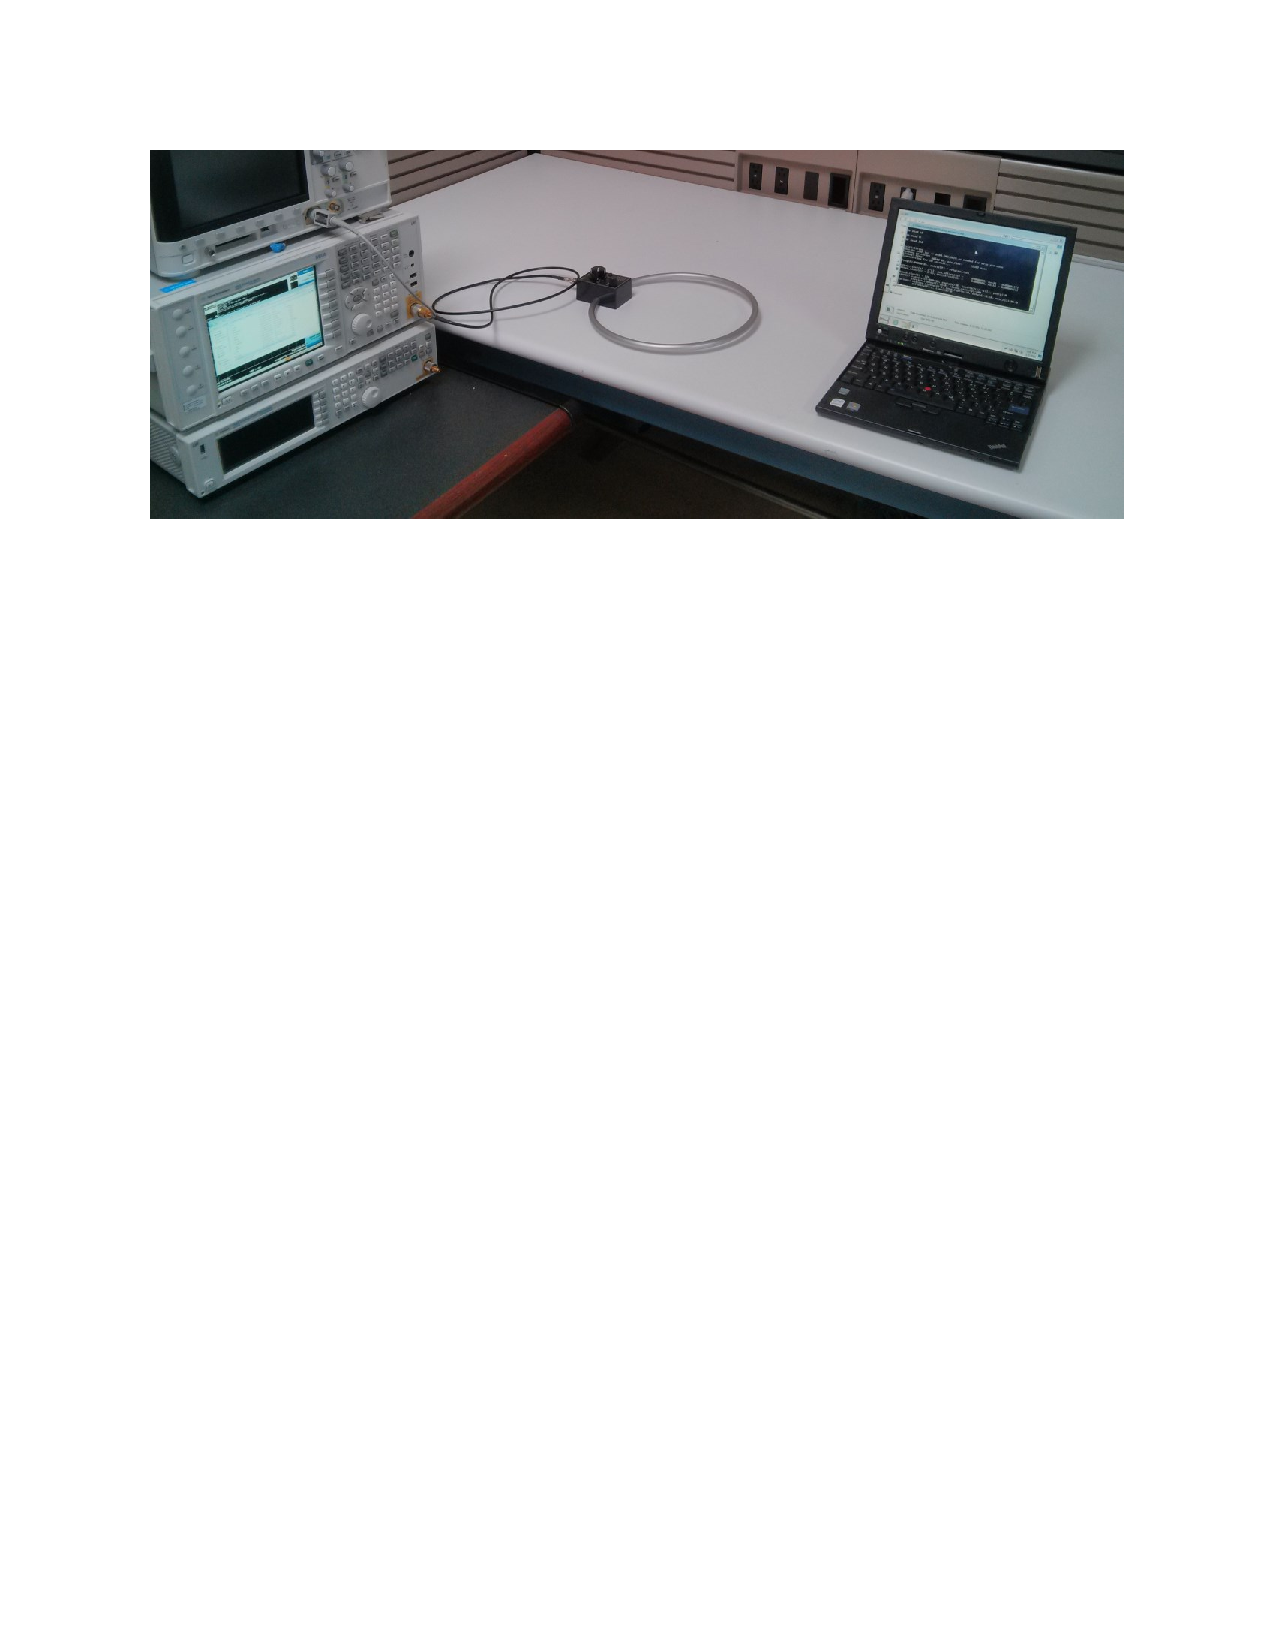
\includegraphics[bb=0.94in 7.49in 7.56in 10.01in,clip=true,width=3.4in]{../TEMC_SAVAT/setup.pdf}
\caption{Measurement setup for the 20 cm loop probe.}
\label{large_setup}
\end{figure}

To conduct a comparison between the x86-based and NIOS-based systems, the probe must pick up emanations from all the parts of the system while at the same time being close enough to pick up the weakest signals tested. A medium sized multiple turn square loop (4 cm width, 20 turns) placed 10~cm above the processor as shown in Figure~\ref{small_setup} was ideal for this purpose. This will be referred to as the 4~cm coil setup. For our measurements the loops are oriented parallel to the PCBs because the magnetic field vectors for the generated signals point in this general direction at the shown probe locations.

\begin{figure}[htb]
\centering
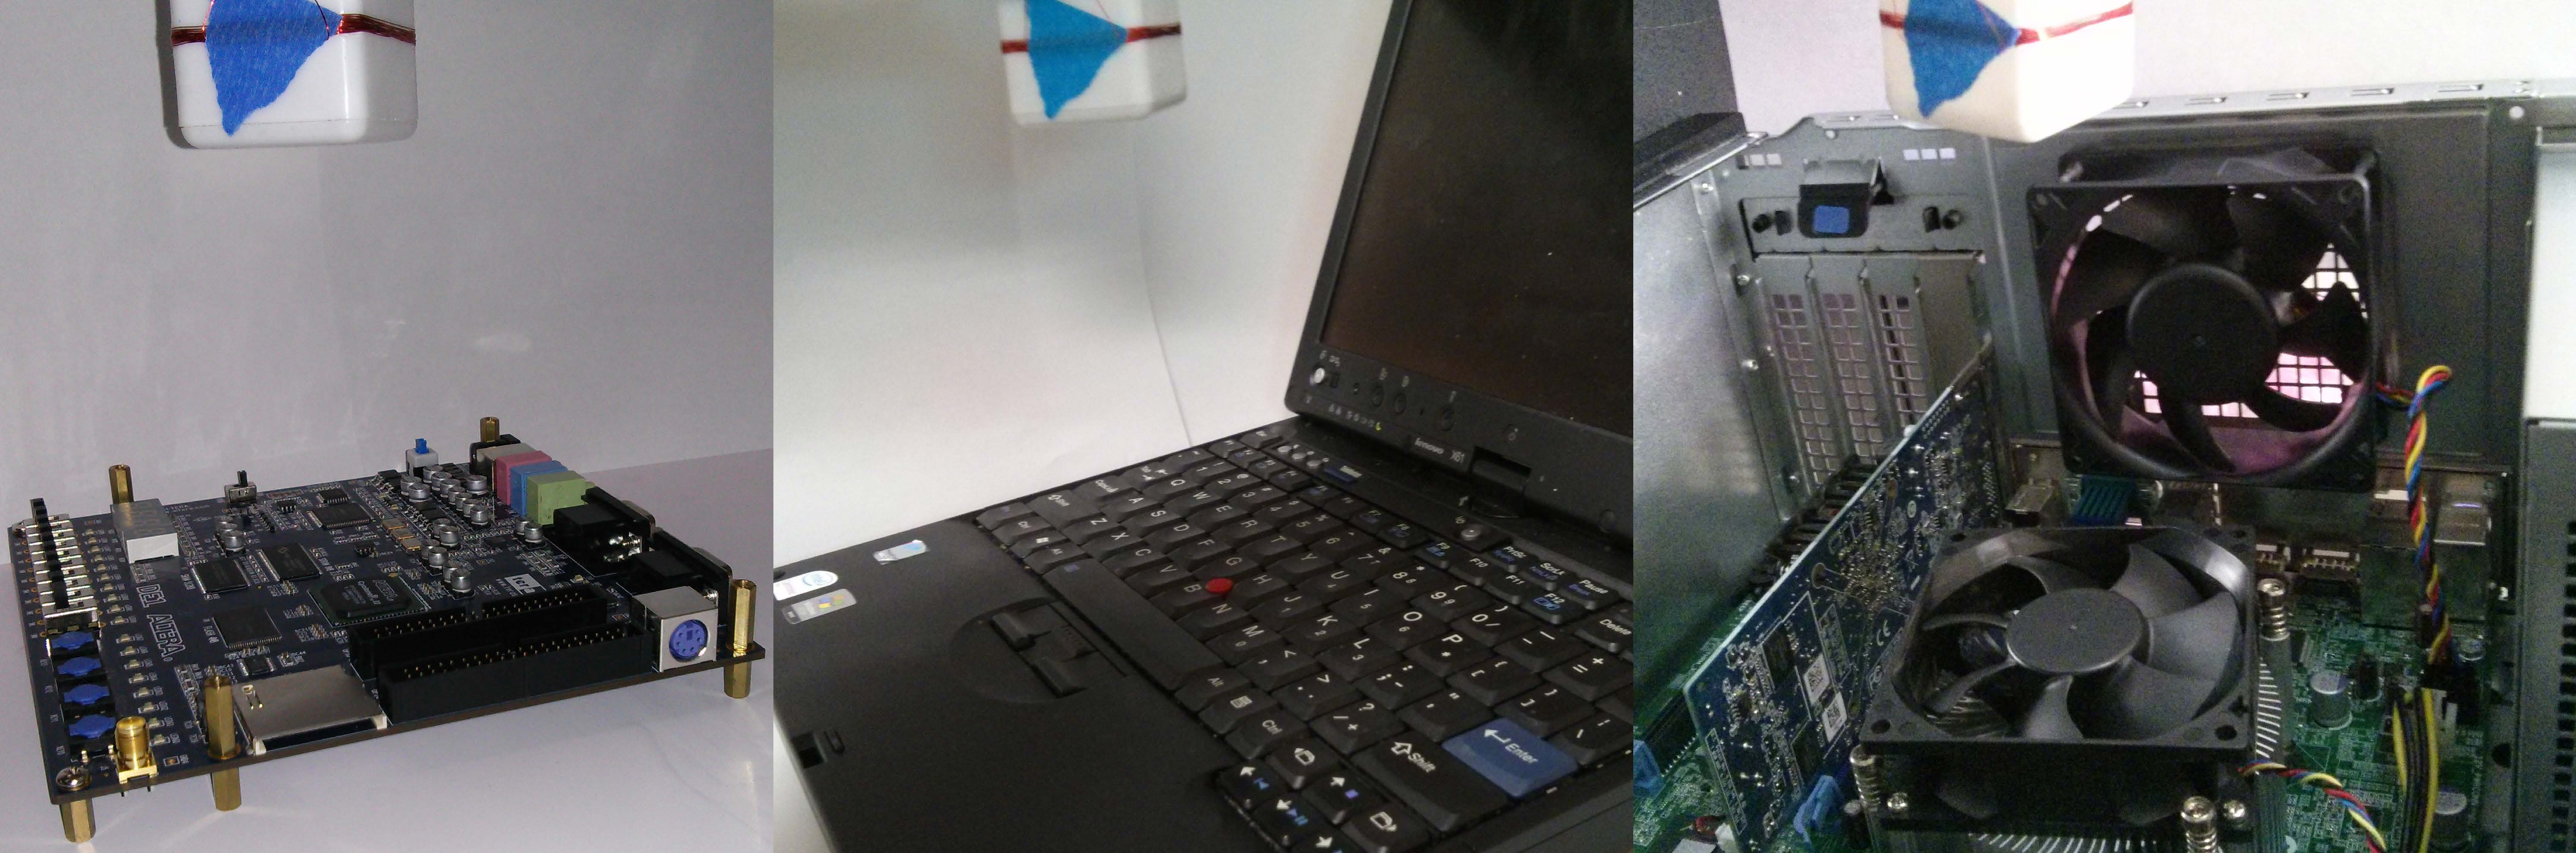
\includegraphics[width=5in]{../emc_comparison_4/setups.pdf}
\caption{FPGA (left), laptop (center), and desktop (right) measurement setups for the 4 cm coil probe.}
\label{small_setup}
\end{figure}

\begin{figure}[htb]
\centering
%\includegraphics[trim=1.4in 5.75in 1.4in 1.2in,clip,width=3.375in]{ADD-LDM-Spectrum.pdf}
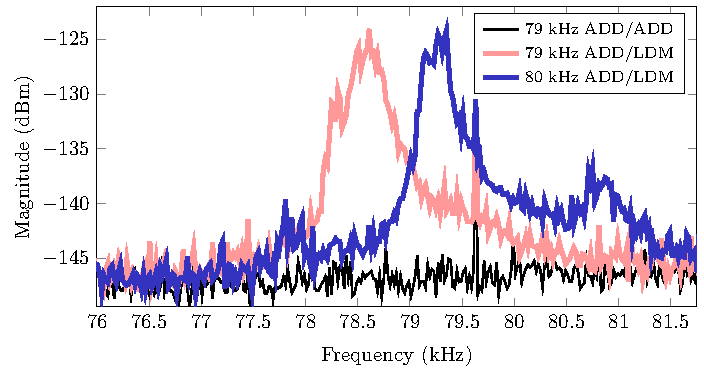
\includegraphics[width=5in]{../TEMC_SAVAT/spect_add_ldm.pdf}
\caption{Power spectrum of ADD/LDM instruction pair at $79$~kHz and $80$~kHz.}
\label{ADD-LDM-Spectrum}
\end{figure}

The power across the probes was measured using a spectrum analyzer (Agilent MXA N9020A). The spectrum around the alternation frequency was re\-cor\-ded with a resolution bandwidth of 1Hz, which results in a very low measurement noise floor because the measured signal is affected only by noise from a 1Hz-wide spectral band. Unless otherwise noted, measurements use an A/B alternation frequency of $80~{\rm kHz}$ and are collected $10~{\rm cm}$ above the device. %explain why
%power calculation?
As shown in Figure~\ref{ADD-LDM-Spectrum}, we can choose the alternation period $T_{alt}$, allowing us to avoid parts of the spectrum where other signals might be present. This spectra shows the ADD/LDM instruction pair (integer addition vs an off-chip memory load) with $79$ and $80$ kHz alternation frequencies along with an ADD/ADD measurement. 

Our measurements include all cases where A and B are the exact same instruction/event, where the resulting A/A alternation should result in no signal at the alternation frequency, such as the ADD/ADD spectrum shown in Figure~\ref{ADD-LDM-Spectrum}. We see that some signal does exist in the band around the intended alternation frequency: these signals may be caused by the instrument's sensitivity floor (which is around $-147$ dBm in Figure~\ref{ADD-LDM-Spectrum}), external radio signals, and a weak signal created by imperfect matching of A/B not-under-test activity. Therefore, these same-instruction alternation measurements give us a very good estimate of the experimental measurement error, and can help identify possible problems such as strong radio interference or mistakes in the A/B alternation code. When A and B instructions/events are not the same, we measure both the A/B alternation and the B/A alternation - these should be the same, so their difference allows us to assess the measurement error caused by placing identical instructions at different program addresses, i.e. the effect of fetch-related variations such as instruction cache alignment.

In Figure~\ref{ADD-LDM-Spectrum}, the $79$ kHz and $80$ kHz ADD/LDM spectra show broad peaks, and these peaks clearly track the alternation frequency. The shifting signals we observe are not due to other unrelated signals (such as nearby switching power supplies, CRT or LCD monitors, or other cabling) because the signal is only present when the A and B instructions differ (i.e. there is no signal for ADD/ADD), and because the observed peak follows the intended alternation frequency. The generated signals are not perfectly concentrated at the intended $f_{alt}$ because (1) $f_{alt}$ cannot be controlled perfectly in a real system and (2) the alternation period $T_{alt}$ (the time to execute one iteration of the outer loop in Figure~\ref{pseudocode}) varies slightly in complex processors and systems, resulting in the dispersion of power around the alternation frequency. For each pair of instructions A and B, we run the A/B microbenchmark and measure the power spectral density from $2.5$ kHz above to $2.5$ kHz below the alternation frequency. Then we integrate over this band to get the total power $P(f_{alt})$ generated by the difference between A and B. Finally the $\textrm{SAVAT}(A,B)$ is calculated from $P(f_{alt})$. 
